\chapter{Geometry reconstruction using constrained nonlinear optimization}\label{ch:optimization}

\vspace{-1.5 em}
\begin{addmargin}[-0.5cm]{0cm}
  \minitoc
\end{addmargin}
\hrule
\vspace{1.5 em}

Much progress was made over the lookup table by treating the geometry reconstruction problem as a constrained nonlinear convex optimization such that MATLAB's \texttt{fmincon} function an be relied on. It relies on trust regions and uses an interior-point algorithm. This worked especially well in the case of triatomic molecules however four-atom systems proved incredibly difficult to tackle here. This was due to the exponential increase in the number of saddle points with dimensionality \footnotemark making the problem highly non-convex and unsuitable for \texttt{fmincon}.

\footnotetext{Recall that triatomic molecules have three degrees of freedom resulting in a problem of dimension 3 while four-atom systems have six. That is, $3N+6$ for an $N$-atom system.}

\section{Mathematical optimization}

We will take a massively expedited tour of mathematical optimization with the aim of explaining the inner workings of the primal-dual interior point methods used for nonlinear constrained optimization in this chapter. To understand how these methods operate, we will need to introduce some important concepts in optimization, namely the duality principle and the Karush-Kuhn-Tucker (KKT) optimality conditions. This is prefaced with a brief introduction to the subject.

No knowledge of mathematical optimization is required, however we will assume some background knowledge throughout this appendix, namely a familiarity with linear algebra, matrix algebra, vector calculus, and some elementary concepts in analysis. \citet{Boyd04} provides an excellent introduction to mathematical optimization, particularly convex optimization, and their freely-available textbook is accompanied by video lectures and lecture slides. However, our problem is nonconvex and so we turn to \citet{Nocedal06} who discuss the more advanced interior-point methods suitable for nonconvex optimization with great clarity.

\subsection{Elementary concepts}
The standard form of a (continuous) optimization problem is
\begin{align} \label{eq:op}
\mathrm{minimize}   \quad & f_0(x) \nonumber \\
\mathrm{subject\;to} \quad &
f_i(x) \leq 0, \; i \in \left\{1, \dots, m \right\}\\
& h_i(x) = 0, \; i \in \left\{1, \dots, p \right\} \nonumber
\end{align}
where $f_0(x): \mathbb{R}^n \rightarrow \mathbb{R}$ is the \emph{objective function} to be minimized over the variable $x \in \mathbb{R}^n$, $f_i(x) \leq 0$ are called the \emph{inequality constraints}, and $h_i(x) = 0$ are called the \emph{equality constraints}. We denote its domain by
\begin{equation}
\mathcal{D} = \bigcap_{i=1}^m \operatorname{dom} f_i \cap \bigcap_{i=1}^p \operatorname{dom} h_i \neq \emptyset
\end{equation}
and assume it is nonempty.

Optimization problems can be classified based on the nature of the objective function and constraints, with each class having their own algorithms. Perhaps the simplest commonly encountered class is \emph{linear programs} where the objective function and constraints are linear, that is $f_0, \dots, f_m, h_1, \dots, h_p$ all satisfy $f_i(\alpha x + \beta y) = \alpha f_i(x) + \beta f_i(y)$ for all $x,y \in \mathbb{R}^n$ and $\alpha, \beta \in \mathbb{R}$. Although no analytical solution exists, efficient algorithms with computation time $\mathcal{O}(n^2m)$ exist to find solutions, such as George Dantzig's simplex method (the one more famous than Nelder-Mead's simplex method discussed in section \ref{sec:nelderMead}).

\emph{Convex optimization problems} are a superset of linear programs and have constraint functions that satisfy $f_i(\alpha x + \beta y) \le \alpha f_i(x) + \beta f_i(y)$ for all $x,y \in \mathbb{R}^n$ and all $\alpha, \beta \in \mathbb{R}$ with $\alpha, \beta \ge 0$ and $\alpha + \beta = 1$. In general, very mature and effective algorithms exist to solve convex optimization problems. If a problem can be transformed into convex form, then it becomes rather easy to solve, however this process can be very difficult and many tricks exist. Least squares problems are actually a special case of convex optimization problems.

\emph{Nonlinear optimization} describes the class of problems where the objective or constraint functions are not linear, but not known to be convex. Unfortunately there are no effective algorithms for solving nonlinear problems in general but there are a number of approaches that may prove fruitful. These include the interior-point method we use and sequential quadratic programming. \citet{Sun15} provide an expository article on ``when nonconvex problem are not scary''.

Unfortunately our problem falls under the umbrella of nonlinear problems. We can describe our objective function as $f_0(x) = |p(x)-p_\textrm{measured}|^2$ where $p(x)$ is the momentum vectors produced following Coulomb explosion of a molecular with structure $x$, and the inequality constraints $f_i(x) \leq 0$ encapsulate the box constraints that limit the geometries recovered to physically reasonable values. For a triatomic molecule, $x = (r_{12}, r_{23}, \theta)$ may be used, for example.

% TODO: Explain: objective function looks like least squares. How is this not convex?

\subsection{Duality}
In order to describe and understand the interior-point method we use, it is neccessary that we look at the concept of duality. We begin by defining the \emph{Langrangian} associated with the optimization problem \eqref{eq:op} as
\begin{equation}
L(x, \lambda, \nu) = f_0(x) + \sum_{i=1}^m \lambda_i f_i(x)
+ \sum_{i=1}^p \nu_i h_i(x)
\end{equation}
where $L: \mathbb{R}^m \times \mathbb{R}^p \rightarrow \mathbb{R}$ and $\operatorname{dom} L = \mathcal{D} \times \mathbb{R}^m \times \mathbb{R}^p$. $\lambda_i$ is the Langrange multiplier associated with the inequality constraint $f_i(x) \leq 0$ and $\nu_i$ is the Langrange multiplier associated with the equality constraint $h_i(x) = 0$. Together, $\lambda \in \mathbb{R}^m$, and $\nu \in \mathbb{R}^p$, are called the \emph{dual variables} or \emph{Langrange multiplier vectors}. The basic idea is that we're accounting for the constraint functions by adjusting the objective function to include a weighted sum of the constraint functions.

The \emph{Lagrange dual function} is defined as the minimum value of the Lagrangian $L$ over $x$
\begin{equation}
g(\lambda, \nu) = \inf_{x \in \mathcal{D}} L(x, \lambda, \nu)
= \inf_{x \in \mathcal{D}} \left[ f_0(x) + \sum_{i=1}^m \lambda_i f_i(x)
+ \sum_{i=1}^p \nu_i h_i(x) \right]
\end{equation}
where $g: \mathbb{R}^m \times \mathbb{R}^p \rightarrow \mathbb{R}$. The $\inf$ operator refers to the \emph{infimum} operator, which may also be called the  \emph{greatest lower bound} operator. An important property of the dual function is that it is concave even when the problem is not convex, as it is the pointwise infimum of a family of affine functions of $(\lambda, \nu)$.

\begin{theorem}
  The Lagrange dual function yields a lower bound on the optimal value of the problem \eqref{eq:op} for $\lambda \succeq 0$ and any $\nu$.
\end{theorem}
\begin{proof}
  Denote the optimal value by $p^\star$ and a feasible point by $x'$ so that it satisfies the constraints $f_i(x') \le 0$ and $h_i(x') = 0$. Then for $\lambda \succeq 0$ and any $\nu$ we have that
  
  $$ \sum_{i=1}^m \lambda_i f_i(x') + \sum_{i=1}^p \lambda_i h_i(x') \le 0 $$
  so that
  $$ L(x',\lambda,\nu) = f_0(x') + \sum_{i=1}^m \lambda_i f_i(x') + \sum_{i=1}^p \lambda_i h_i(x') \le f_0(x') $$
  and
  $$ g(\lambda, \nu) = \inf_{x \in \mathcal{D}} L(x, \lambda, \nu) \le L(x', \lambda, \nu) \le f_0(x') $$
  which must hold for every feasible point $x'$ including the optimal solution $x^\star$ and thus
  $$ g(\lambda, \nu) \le p^\star = f_0(x^\star) $$ 
\end{proof}


As the lagrange dual function provides a lower bound on the optimal value $p^\star$ that depends on $(\lambda,\nu)$, we may be interested in finding the best lower bound. This leads to the \emph{Lagrange dual problem} associated with \eqref{eq:op} which can be stated as
\begin{align} \label{eq:dualop}
\mathrm{maximize}    \quad & g(\lambda, \nu) \nonumber \\
\mathrm{subject\;to} \quad & \lambda \succeq 0
\end{align}
and is always a convex problem as the dual function $g(\lambda, \nu)$ is always convex as mentioned when we introduced it. We can then talk about \emph{dual feasible} pairs $(\lambda,\nu)$ with $\lambda \succeq 0$ and $g(\lambda,\nu) > -\infty$, \emph{optimal Lagrange multipliers} or the \emph{dual optimal} pair $(\lambda^\star, \nu^\star)$, and the optimal value of the dual problem, denoted $d^\star$ . In some contexts involving both the dual problem \eqref{eq:dualop} and the original problem \eqref{eq:op}, the original problem is called the \emph{primal problem}.

If the optimal value of the dual problem $d^\star$ and of the primal problem $p^\star$ are equal, $d^\star = p^\star$, then we say that \emph{strong duality} holds and the \emph{optimal duality gap} is zero, $d^\star - p^\star = 0$. Otherwise $d^\star \le p^\star$ and we say that \emph{weak duality} holds.

\subsection{Optimality conditions}
It will be quite useful to impose conditions on what makes a feasible point an optimal point or solution for both the primal and dual problems. Denoting the optimal primal solution by $x^\star$ and the optimal value by $p^\star = f_0(x^\star)$, we already know that it must satisfy the constraints $f_i(x^\star) \ge 0$ and $h_i(x^\star) = 0$. Denoting the dual optimal by $(\lambda^\star, \nu^\star)$ we would like for $\lambda_i^\star \ge 0$ so that the dual function provides a lower bound on $p^\star$. 

% TODO: Complementary slackness

Since $x^\star$ minimizes the Lagrangian $L(x, \lambda^\star, \nu^\star)$ over $x$, its gradient must be zero at the minima or maximum $x^\star$, giving us
\[
\nabla f_0(x^\star) + \sum_{i=1}^m \lambda_i^\star \nabla f_i(x^\star)
+ \sum_{i=1}^p \nu_i^\star \nabla h_i(x^\star) = 0
\]

Together, we can summarize the five conditions we obtained
\begin{align} \label{eq:kkt}
f_i(x^\star) & \geq 0, \; & i & \in {1,\dots,m} \nonumber \\
h_i(x^\star) & = 0, \; & i & \in {1,\dots,p} \nonumber \\
\lambda_i^\star & \geq 0, \; & i & \in {1,\dots,m} \\
\lambda_i^\star f_i(x^\star) & = 0, \; & i & \in {1,\dots,m} \nonumber \\
\nabla f_0(x^\star) + \sum_{i=1}^m \lambda_i^\star \nabla f_i(x^\star)
+ \sum_{i=1}^p \nu_i^\star \nabla h_i(x^\star) & = 0, \; & i & \in {1,\dots,m} \nonumber
\end{align}
which together are called the \emph{Karush-Kuhn-Tucker (KKT) conditions}. They are sometimes referred to as the first-order optimality conditions, and second-order conditions do exist.

\subsection{Trust regions}
Switching gears a little bit, we'll look at a general strategy of solving optimization problem using the concept of a \emph{trust region}. When searching for an optimal solution starting from an initial point $x_0$, the idea is to create and solve an approximate optimization problem at each iterate $x_k$ with the hope that the approximation is easier to solve yet locally accurate enough to help locate the true optimal solution. The approximated is \emph{trusted} only so much, up to some radius or region boundary. A circular or spherical trust region may be used, but so can box and elliptical regions. If a sufficiently better iterate $x_{k+1}$ is not found within the trust region then the region may be shrunk in case the approximation is invalid so far from the iterate $x_k$.

The approximation employed may be termed the \emph{model function} so that the approximate problem at iterate $x_k$ becomes $\operatorname{minimize}_p m_k(x_k + p)$ where $p$ is the candidate step so that $x_k + p$ lies within the trust region. A very popular model function takes the form of a quadratic approximation using the first two terms of a Taylor approximation of the objective function at the iterate point
\begin{equation}
  m_k(x_k + p) = f(x_k) + p^T \nabla f(x_k) + \frac{1}{2} p^T \nabla^2 f(x_k) p
\end{equation}
where $\nabla f(x_k)$ and $\nabla^2 f(x_k)$ are the gradient and Hessian of the objective function $f$ at the point $x_k$ \citep{More83}.

Trust regions see a great deal of use in nonlinear optimization methods, and can be modified for constrained optimization. Beyond the choice of approximation and trust region type, choosing the region size and shape, the step size, and the method used to solve even the trust region subproblem are important. Another class of methods serving a similar purpose are line search methods where a direction is first chosen to search for the next iterate, so that the step size is chosen second. Line search methods are in a sense the dual of trust region methods, where the step size (trust region radius or boundary) is chosen first, then a direction is chosen.

\subsection{Primal-dual interior point methods}
The idea behind an interior-point method is to modify the an original problem to take into account the constraint functions by modifying the objective function to penalize iterates that leave the feasible region (or break the constraints). As this may modify the optimal solution, the approximation is realxed as a local minimum is approached, so you are essentially solving a series of approximate optimization subproblems. A very popular approximation is to use a logarithmic barrier, that induces a penalty that approaches $\infty$ as you approach the constraint.

\begin{align}
\mathrm{minimize} \quad & f_\mu(x,s) = f(x) - \mu \sum_{i=1}^{m} \ln s_i \nonumber \\
\mathrm{subject\;to} \quad & g_i(x) + s_i = 0 \\
                           & h_i(x) = 0 \nonumber
\end{align}

Direct step
\begin{equation}
\begin{pmatrix}
  H   & 0        & J_h^T & J_g^T \\
  0   & S\Lambda & 0     & -S \\
  J_h & 0        & I     & 0 \\
  J_g & -S       & 0     & I
\end{pmatrix}
\begin{pmatrix}
  \Delta x  \\
  \Delta s  \\
  -\Delta y \\
  -\Delta \lambda \\
\end{pmatrix}
=
\begin{pmatrix}
\nabla f - J_h^T y - J_g^T \lambda  \\
S\Lambda - \mu e \\
h \\
g + s \\
\end{pmatrix}
\end{equation}
where $H$ is the Hessian of the Lagrangian of $f_\mu$
\begin{equation}
H = \nabla^2 f(x) + \sum_i \lambda_i \nabla^2 g_i(x) + \sum_j \lambda_j \nabla^2 h_j(x),
\end{equation}
$J_g$ and $J_h$ are the Jacobians of the constraint function $g$ and $h$ respectively, $S = \operatorname{diag}(s)$, $\Lambda = \operatorname{diag}(\lambda)$, $\lambda$ and $y$ are the Lagrange multipliers associated with the constraint functions $g$ and $h$ respectively, and $e$ is a vector of ones with the same size as $g$.


\subsection{Curse of dimensionality and possible solutions}
The curse of dimensionality, a term first introduced by \citet{Bellman57} when considering problems in dynamic optimization, refers to the exponential increase in volume when adding extra dimensions to Euclidean space \citep{Keogh10}. It manifests itself in two ways when tackling the geometry reconstruction problem for larger and larger molecules, as we need $3N-6$ parameters to describe the geometry of an molecule with $N \ge 3$ atoms. Firstly, the parameter space or phase space to be searched increases exponentially with $N$, and with this increase may come an increase in local minima, and possible an increase in the number of degenerate geometries. While we believe, anecdotally, that interior-point methods will still be feasible for polyatomic molecules with several atoms, convergence will definitely take longer and multiple runs may be required before finding a feasible geometry or any degenerate geometries, possibly necessitating the use of a supercomputer cluster.

The second manifestation, which seems more severe from preliminary investigations of reconstructing acetylene (\ch{C2H2}) molecular geometries, is the proliferation of saddle points in high-dimensional spaces, termed the \emph{saddle-point problem} as argued by \citet{Pascanu14} using evidence from statistical physics, random matrix theory, and neural network theory. Fortunately, this is a very active area of research due to the recent surge and revival of interest in artificial intelligence \citep{Bengio16,LeCun15} and the development of new algorithms may be helpful in reconstructing larger molecules. One recent example worth looking into for future improvements include the saddle-free Newton method proposed by \citet{Dauphin14} which uses second-curvature information to rapidly escape from high-dimensional saddle points.

One easy method of tackling this problem when attempting to reconstruct larger molecules is to fix certain parameters of the molecule's geometry, ones which may exhibit very low variability. An example may be the triple \ch{C+C} bond in acetylene.

\section{Implementation}
As we mentioned in the previous section, there are many complications involved with implementing advanced optimization algorithms such as interior-point methods and so instead of reinventing the wheel, we will use a readily-available and mature implemention in MATLAB's Optimization Toolbox in conjunction with the Global Optimization and Parallel Processing Toolboxes. In the spirit of open science and reproducibility, we would have chosen an open-source implementation however this was not a consideration at the beginning of this study and the MATLAB implementation seems to be superior to most of the available alternatives we inspected, commericial and otherwise.

The MATLAB Optimization Toolbox provides a general-purpose nonlinear programming solver, \texttt{fmincon}, that attempts to find the minimum of a constrained nonlinear multivariable function. Among the algorithms it can employ is the interior-point method we described in the previous section.  We use \texttt{fmincon} to find geometries and provide it with \emph{box constraints} to ensure we recover triatomic geometries with the constraints that $\SI{100}{\pico\meter} \le r_\mathrm{CO}, r_\mathrm{CS} \le \SI{500}{\pico\meter}$ and $\SI{140}{\deg} \le \theta \le \SI{180}{\deg}$.

We describe the bond lengths in picotmeters ($10^{-12}$ m) and the bond angles in units of degrees to keep all the parameters within the same order of magnitude as opposed to 12 orders of magnitude apart if we used meters and degrees. This seemed to be especially important for \texttt{fmincon} as it performed much better, converging on the correct solution more often and in fewer iterations, when the parameters were all numerically within the same order of magnitude. This is because the step sizes and trust region radii chosen by the interior-point algorithm depend on the values of the Hessian and Jacobian which may take on extreme values when the derivatives of the objective function are very small or very large as may be the case when the input vary in magnitude by 12 orders.  A more visual description would to be imagine finding an optimal point within a region described by a cube in phase space when using picometers and degrees, and finding an optimal point within an almost infinitesimally thin sheet in phase space when using meters and degrees.

To find degenerate geometries and ensure that we have found geometries corresponding to global minima and not just local minima, we run \texttt{fmincon} multiple times for each set of measured momentum vectors, each time using a different initial starting point. This is done using the \texttt{MultiStart} solver from the Global Optimization Toolbox which runs multiple instances of \texttt{fmincon} in parallel using a uniformly distributed set of starting points in an attempt to find multiple solutions. Typically only a single run is required to find a solution, especially when using simulated data, but at least several runs may be needed before finding a second degenerate geometry.

As we may have many measurements to reconstruct, we may want to make use of all available processor cores when running on a personal computer and we especially want to make full use of each core when running on a supercomputer cluster, so the measurements are iterated over using a \emph{parallel for loop} or a \texttt{parfor} loop which executes each loop iteration on a different core. When the number of cores exceeds the number of \texttt{fmincon} runs required by \texttt{MultiStart}, this ensures that the other cores are reconstructing other geometries.

\section{Reconstructions of experimental data}
Now that we have a more sophisticated method for reconstructing geometries, we should reconstruct the same geometries we saw in section \ref{sec:degenerateGeometries} for the \ch{OCS} $(2,2,2)$ molecule.

\begin{figure}
  \centering
  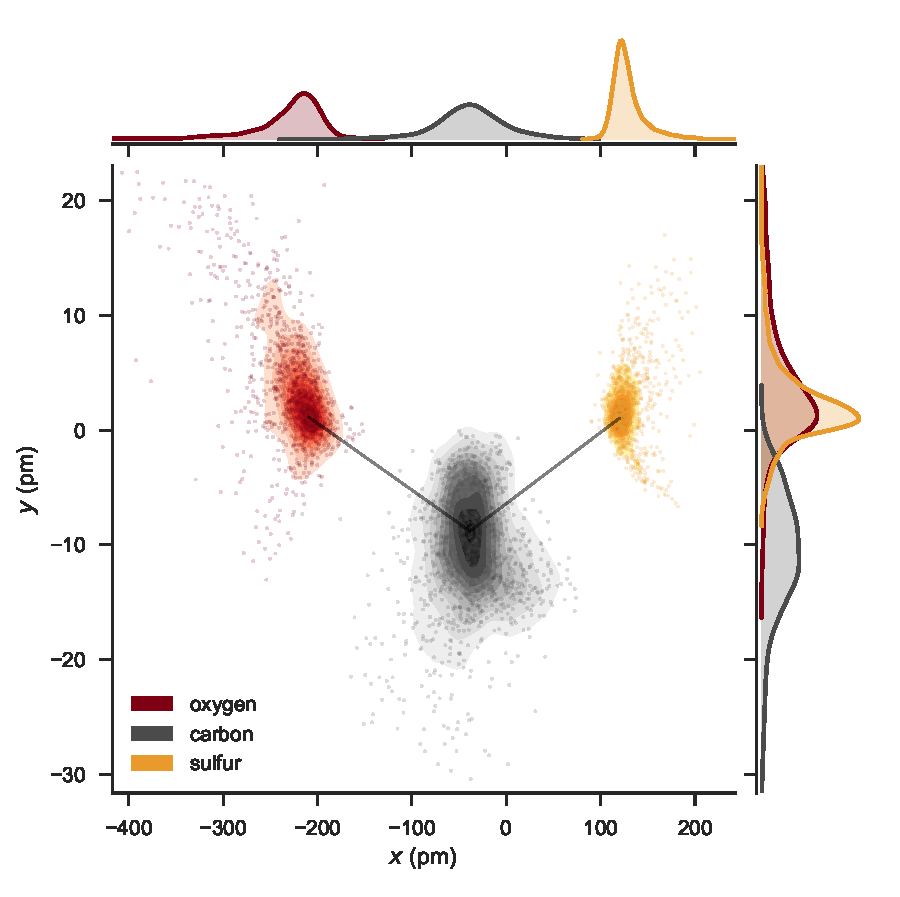
\includegraphics[width=\textwidth]{Plots/OCS2227fsMOGeometry}
  \caption[Scatter plot showing a reconstruction of the molecular geometry of \ch{OCS} following Coulomb explosion by a \SI{7}{\fs} laser pulse for the $(2,2,2)$ fragmentation channel.]
  {Scatter plot showing a reconstruction of the molecular geometry of \ch{OCS} following Coulomb explosion by a \SI{7}{\fs} laser pulse for the $(2,2,2)$ fragmentation channel. Each geometry is represented by three colored points, one for each atomic fragment; red for oxygen on the left, black for carbon in the center, and yellow for sulfur on the right. The colors were chosen to imitate the CPK coloring convention. Geometries are plotted such that the molecule's center of mass is at the origin to showcase the variance in each atomic fragment's position, and are rotated such that a vertical line bisects the \ch{O-C-S} bond angle. Bivariate kernel density estimates (KDE) with a Gaussian kernel, plotted as shaded-in contours, are used to estimate the the probability density of each atomic fragment's position (see section \ref{sec:kde} for a discussion of KDE's). Solid black lines are drawn between the peaks of each atomic fragment's kernel density estimate to illustrate the \emph{modal geometry} or most likely geometry. Along the top of the plot, univariate KDE's show the probability density of each atomic fragment's position along the $x$-axis, and the same is done for the $y$-axis along the right. The molecule is almost straight but an aspect ratio of approximately $10:1$ is employed to showcase variability in the $y$-axis.}
  \label{fig:OCS2227fsMOGeometry}
\end{figure}

\subsection{Comparision with the lookup table}
Qualitatively not very different.

\subsection{Investigating individual reconstructions}
While figure \ref{fig:OCS2227fsMOGeometry} gives a good intuitive image of what a molecular geometry looks like, it would be interesting to see a distribution of bond lengths and bond angles and quantify the variable in each of these parameters. We could also look at correlations between the bond lengths and bond angles and see, for example, if longer \ch{C-O} bond lengths correspond to longer \ch{C-S} bond lengths, or if more bent geometries tend to have longer bond lengths. To visualize this relationship in figure \ref{fig:OCS2227fsMOGeometryPairs} we utilize a scatterplot matrix as we did for figure \ref{fig:OCS2227fsMomentum}.

\begin{figure}
  \centering
  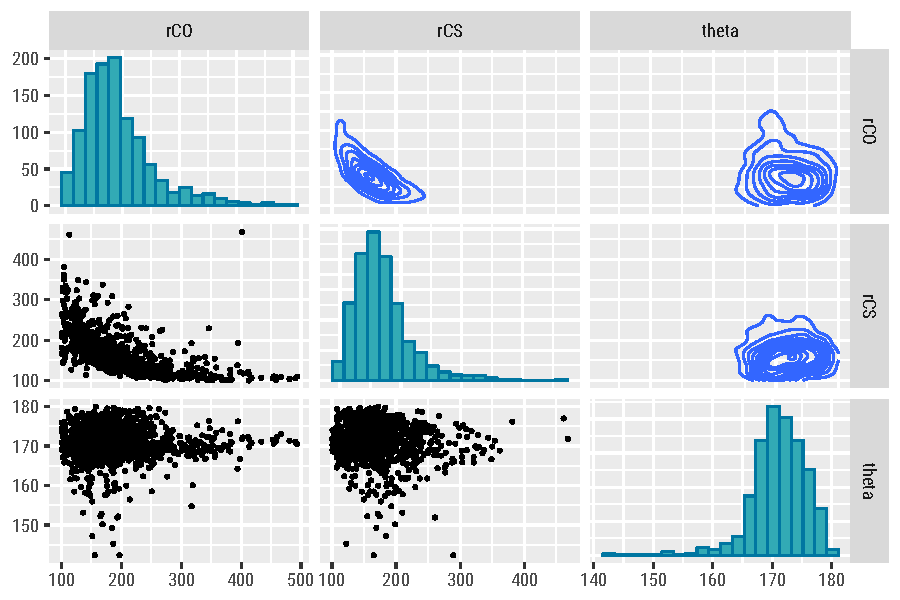
\includegraphics[width=\textwidth]{Plots/OCS2227fsMOGeometryPairs}
  \caption[Scatter plot matrix showing the bivariate relationship between the parameters $(r_\mathrm{CO}, r_\mathrm{CS}, \theta)$ for the reconstructions of the molecular geometry of \ch{OCS} following Coulomb explosion by a \SI{7}{\fs} laser pulse for the $(2,2,2)$ fragmentation channel.]
  {Scatter plot matrix showing the bivariate relationship between the parameters $(r_\mathrm{CO}, r_\mathrm{CS}, \theta)$ for the reconstructions of the molecular geometry of \ch{OCS} following Coulomb explosion by a \SI{7}{\fs} laser pulse for the $(2,2,2)$ fragmentation channel. On the diagonal, histograms show the distribution of bond lengths and bond angle for the reconstructed geometries (tick marks at the bottom of each column). Below the diagonal, scatter plots show the bivariate relationship between each molecular parameter. Above the diagonal, the same relationship is given using a contour plot instead.}
  \label{fig:OCS2227fsMOGeometryPairs}
\end{figure}

The bond length distributions on the diagonal of figure \ref{fig:OCS2227fsMomentum} make sense; they peak slightly above the equilibrium values indicating some molecular rearrangement and bond lengthening due to the molecule's interaction with the laser field. The bond angle distribution shows less variability suggesting that the molecule may have not had much time to bend yet. % TODO: How similar is this to theoretical calculations?

What is very interesting, however, is the relationship between the two bond lengths, $r_\mathrm{CO}$ and $r_\mathrm{CS}$. We may expect both bond lengths to lengthen or possibly to have one bond stretch while the other remains relatively constant, but the reconstructions actually indicate the complete opposite, that while one stretches the other bond shrinks almost following a reciprocal relationship. This effect becomes even more pronounced when reconstructed molecular geometries exposed to longer pulse lengths.

Certainly such bizarre data suggests that something must have gone wrong. To our knowledge no other studies performing geometry reconstruction using Coulomb explosion imaging have reported the correlations between their bond lengths and bond angles, so it is impossible to tell whether other studies have found similar relationships or if we have done something wrong.\footnotemark~ When plotted, the geometries and even the bond length and bond angle distributions make physical sense, it is only the correlations that do not.

\footnotetext{Private communication with collaborators suggests that other investigations have led to similar worrying results, leading to the abandonment of geometry reconstruction efforts.}

Such worrying results force us to distrust the geometry reconstructions we have done so far. While the average geometries and overall dataset may look fine, the individual geometries seem to not make physical sense so the dataset cannot be trusted. It is worth noting that performing a similar analysis on the geometries reconstructed using the lookup table produces the same worrying results so this bizarre relationship seems to emerge out of at least two different reconstruction methods. We will come back and resolve this issue in the next chapter (the reconstruction method is not at fault).

\section{Investigating degenerate geometries}
We should also test whether this approach can accurately reconstruct simulated geometries as we tested the Nelder-Mead simplex method in section \ref{ssec:simplexFail} and the lookup table in section \ref{ssec:LTaccuracy}. We will also use this information to actually investigate degenerate geometries a bit more closely.

When testing the accuracy of the Nelder-Mead simplex method and the lookup table, we did not do it so thoroughly. We just varied one molecular parameter at a time, which was sufficient to show the inadequecy of the simplex method. For a more thorough test, we will substantially vary all the parameter but simulating the Coulomb explosion of geometries within a cube in phase space described by $\SI{100}{\pico\meter} \le r_\mathrm{CO}, r_\mathrm{CS} \le \SI{500}{\pico\meter}$ and $\SI{140}{\deg} \le \theta \le \SI{180}{\deg}$. For a low-resolution testing, we pick geometries $r_\mathrm{CO} \times r_\mathrm{CS} \times \theta_\mathrm{OCS}$ where $r_\mathrm{CO}$ and $r_\mathrm{CS}$ are sets containing $10$ uniformly spaced bond lengths between \SI{100}{\pico\meter} and \SI{500}{\pico\meter}, $\theta_\mathrm{OCS}$ is a set containing $10$ uniformly spaced bond angles between \SI{140}{\deg} and \SI{180}{\deg}, and $X \times Y = \lbrace (x,y) | x \in X \;\mathrm{and}\; y \in Y \rbrace$ denotes the cartesian product as expressed in set-builder notation \citep[p. 6]{Warner90}. Thus we are reconstructing $10^3 = 1000$ geometries from simulated Coulomb explosions.

We find that the optimization routine can reconstruct the simulated geometries in $98.8\%$ of cases using only a single starting guess. Each reconstruction takes approximately one second. In each of these reconstructions, the parameters of the recovered geometry numerically matched the original geometry up to several decimal places. The absolute error between the recovered and simulated momentum vectors was below $10^{-55}$ for $95\%$ of reconstructions, with the mean error being approximately $10^{-57}$ which is 10 orders of magnitude lower than the absolute errors on momentum vectors retreived using the lookup table. Since we use the square of the $\ell_2$-norm to quantify the absolute error, this actually represents an improvement of approximately 5 orders of magnitude in accuracy over the lookup table. Using multiple starting points recovers geometries for the other $1.2\%$ of cases.

While the optimization routine recovered very precise geometries whose post-explosion momentum vectors very closely match the expected vectors, the geometries were not always the ones we started with and expected. It seems that in about $5\%$ of cases, the routine returned a degenerate geometry. It is important to note that when the Nelder-Mead simplex method and the lookup table returned a different geometry than expected, it was just a failure in recovering the exact geometry as the momentum vectors did not match closely except for a small number of cases where it had found a degenerate geometry. However, in this case we are getting very precise reconstructions and each different geometry represents a degenerate geometry. To showcase the nature of these degenerate geometry, we plot arrows between the expected geometry and the recovered degenerate geometry in figure \ref{fig:OCS222DegeneracyMapSD}, which we will call a \emph{degeneracy map}. If the recovered geometry was the original geometry as expected, then no arrow is plotted.

\begin{figure}
  \centering
  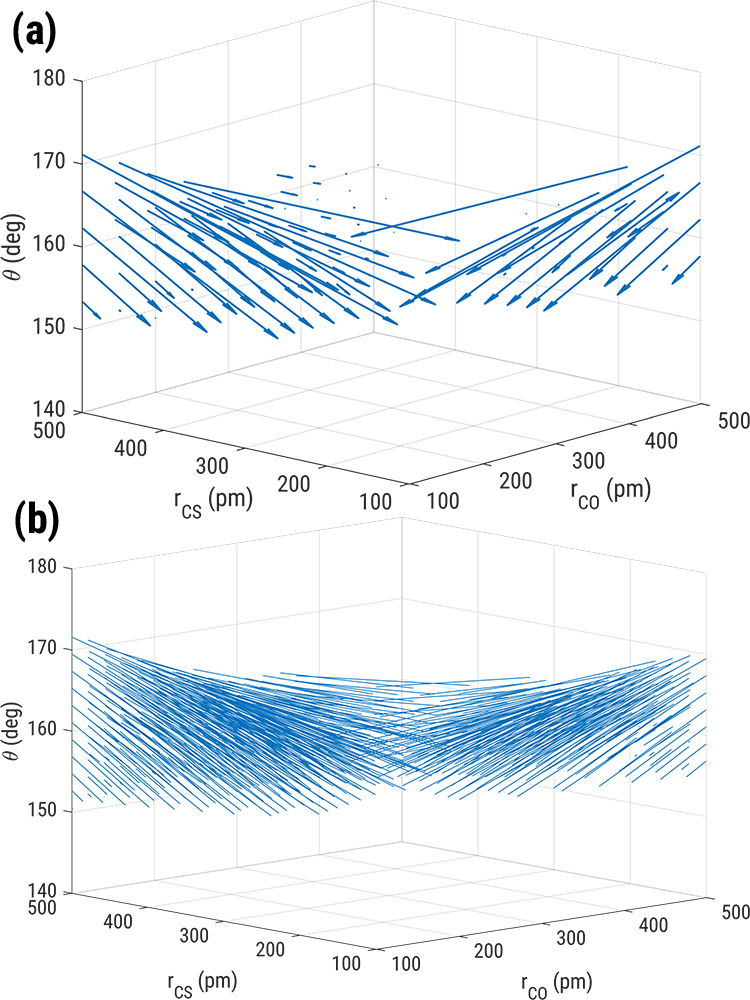
\includegraphics[width=\textwidth]{Plots/OCS222DegeneracyMap}
  \caption[Mapping between degenerate geometries for the \ch{OCS} $(2,2,2)$ molecule.]
  {Mapping between degenerate geometries for the \ch{OCS} $(2,2,2)$ molecule. The Coulomb explosion of $1000$ uniformly distributed geometries within a cube in phase space described by $\SI{100}{\pico\meter} \le r_\mathrm{CO}, r_\mathrm{CS} \le \SI{500}{\pico\meter}$ and $\SI{140}{\deg} \le \theta \le \SI{180}{\deg}$ was simulated and then reconstructed using the momentum vectors of the atomic fragments that resulted from the simulations. If the reconstructed geometry matched the original geometry exactly, then no arrow is plotted. However, an arrow is plotted from the original expected geometry to the recovered geometry if it represented a degenerate geometry. Arrows small enough that they resemble points indicate a slight numerical difference between the expected geometry and the reconstructed geometry, but do not neccessarilly represent a degenerate geometry.}
  \label{fig:OCS222DegeneracyMapSD}
\end{figure}

We see some patterns in the degenerate geometries recovered. They only occur for molecules with bond angles between approximately \SI{150}{\deg} and \SI{170}{\deg} which includes a sizable minority of the molecules reconstructed as indicated by the bond angle distribution in figure \ref{fig:OCS2227fsMOGeometryPairs}. Degenerate geometries exist mainly for molecules exhibiting significant bond asymmetry and these geometries tend to be degenerate with another molecule that is more bent and has a smaller degree of bond length asymmetry. They also seem to appear in two regions, one where the \ch{C-O} bond length is longer, and another where the \ch{C-S} bond length is longer. Figure \ref{fig:OCS222DegeneracyMapSD} may suggest the existence of a discrete number of these degenerate geometries, however, repeating the test with a greater number of geometries produces very similar results except for a correspondingly higher density of arrows, suggesting that regions exist in phase space where every geometry is degenerate with another, \ie~ that an uncountably infinite\footnotemark~ number of degenerate geometries exist.

\footnotetext{A countably finite set may refer to the set of integers $\mathbb{Z} = \lbrace 0, \pm 1, \pm 2, \dots \rbrace$, for example, which may be enumerated. An uncountably infinite set has the same cardinality as the set of real numbers $\mathbb{R}$ which cannot be enumerated \citep{Halmos17}.}

In these simulations we knew \textit{a priori} what geometry we expected to reconstruct, so we can assign a direction to each arrow. However, when reconstructing experimental data, we have no prior knowledge of what geometry we expected to recover, so the arrow could point in either direction. In some cases it might be possible to choose one degenerate geometry over the other(s) if one is physically unrealistic, \eg~ if it is very highly bent or exhibits an extreme bond length asymmetry.

\begin{figure}
  \centering
  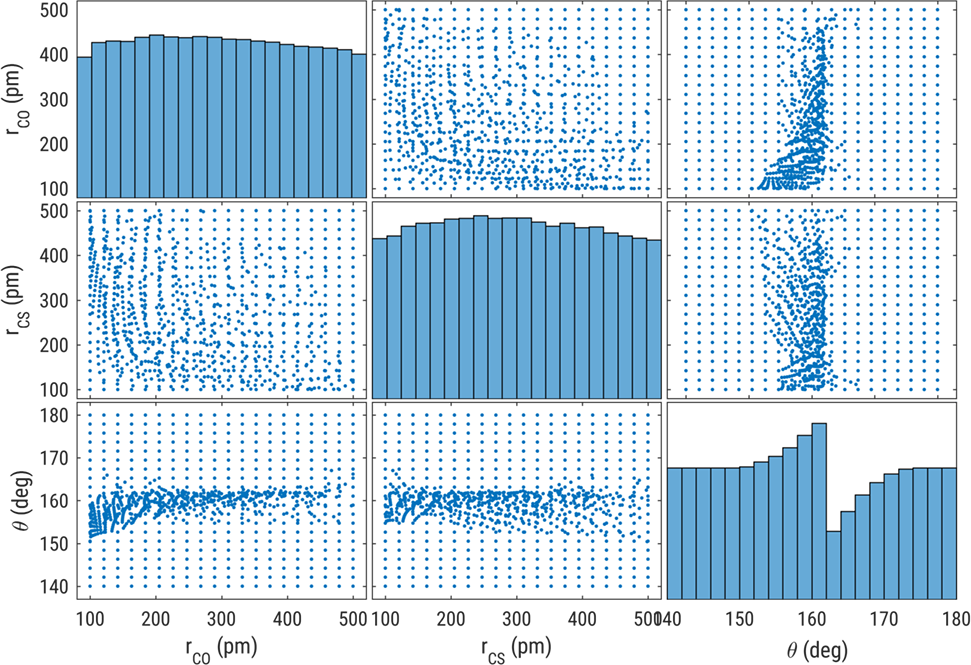
\includegraphics[width=\textwidth]{Plots/OCS222DegeneracyMapHDPairs}
  \caption[Scatter plot matrix showing the bivariate relationship between the parameters $(r_\mathrm{CO}, r_\mathrm{CS}, \theta)$ for the reconstructions of the molecular geometry of \ch{OCS} from momentum vectors obtained from simulated Coulomb explosions.]
  {Scatter plot matrix showing the bivariate relationship between the parameters $(r_\mathrm{CO}, r_\mathrm{CS}, \theta)$ for the reconstructions of the molecular geometry of \ch{OCS} from momentum vectors obtained from simulated Coulomb explosions of $8,000 \; (20^3)$ uniformly distributed geometries within a cuboid in phase space described by $\SI{100}{\pico\meter} \le r_\mathrm{CO}, r_\mathrm{CS} \le \SI{500}{\pico\meter}$ and $\SI{140}{\degree} \le \theta \le \SI{180}{\degree}$. On the diagonal, histograms show the distribution of bond lengths and bond angle for the reconstructed geometries with tick marks at the bottom of each column (no vertical scale is given for the histograms). Below the diagonal, scatter plots show the bivariate relationship between each molecular parameter. Above the diagonal, the same scatter plots are shown with the $x$ and $y$-axes interchanged to correspond with the axes labels and tickmarks.}
  \label{fig:OCS222DegeneracyMapHDPairs}
\end{figure}

To further visualize the set of geometries we recovered, we utilize a scatterplot matrix in figure \ref{fig:OCS222DegeneracyMapHDPairs} showing the bond length and angle distributions as well as their bivariate relationships. This uses $8,000$ geometries. It is interesting to note that whenever degenerate geometries exist, the more bent geometry is found. Perhaps these more bent solutions posess a larger \emph{basin of attraction}, which may or may not be strongly dependent on the optimization algorithm employed. It might be interesting to visualize them, possibly taking a similar approach as \citet{Asenjo13} who actually employ mathematical optimization methods to determine energy minimizing molecular structures. They observe basins with rather complicated boundaries, reminiscent of the beautiful and spatially chaotic patterns produced by the magnetic pendulum.

For the feasibility of geometry reconstruction, however, this result carries extra worries. Even when the measured momentum vectors can be mapped to a molecular geometry very precisely, the existance of multiple solutions corresponding to very different geometries may make it impossible to perform accurate geometry reconstructions, especially when multiple degenerate geometries represent physically realizable geometries.

Interestingly, we find that we recover degenerate geometries approximately $5\%$ of the time while \citet[supplementary information]{Kunitski15} report finding degenerate geometries approximately $10\%$ of the time, although they chose to disregard them for their analyses.

We considered whether these degeneracies could arise due to our choice of momentum convention in section \ref{sec:conventions} however our convention simply rotates the three momentum vectors such that the carbon's momentum vector lies along the $+x$-axis and all three momentum vectors lie in a plane.

\section{Conclusions}
\emph{The importance of covariances and joint distributions}---

\emph{Geometry reconstruction is highly sensitive to uncertainty in the momentum vectors}---

\subsection{Future directions}